\documentclass[12pt]{article}
\usepackage[a4paper,left=1in,right=1in,top=1in,bottom=1in]{geometry}
\usepackage[utf8x]{inputenc}
\usepackage{gensymb}
\usepackage{indentfirst}
\usepackage{graphicx}
\graphicspath{{/home/dnehme/Dropbox/profissional/protocolos/ptc-validation-roms/ssh/figure/}}
\usepackage[abs]{overpic}
\usepackage{float}
\usepackage[brazil]{babel}
\usepackage{multirow}
\usepackage{lmodern}
\usepackage{titlesec}
\usepackage{xcolor}
\usepackage{natbib}

\setcounter{secnumdepth}{4}

\titleformat{\paragraph}
{\normalfont\normalsize\bfseries}{\theparagraph}{1em}{}
\titlespacing*{\paragraph}
{0pt}{3.25ex plus 1ex minus .2ex}{1.5ex plus .2ex}


\begin{document}

\begin{center}
	{\bf {\Large Protocolo de validação de simulações do ROMS}}
	\vspace{5mm}\par

	{\bf {\large Elevação da Superfície Livre}}
	\\
	\hrulefill
	\\
	
	{\bf Equipe:} {\it Douglas M. Nehme}\\
	\par
\end{center}

\tableofcontents

\newpage

\addcontentsline{toc}{section}{Apresentação}
\section*{Apresentação}
	\par A
	
\section{Variáveis obtidas por satélite}

	\begin{itemize}
		\item Elevação da Superfície Livre (\textit{Sea Surface Height} - SSH): Os altimetros medem a 
	\end{itemize}Elevação da Superfície Livre

	\begin{figure}[h]
		\centering
		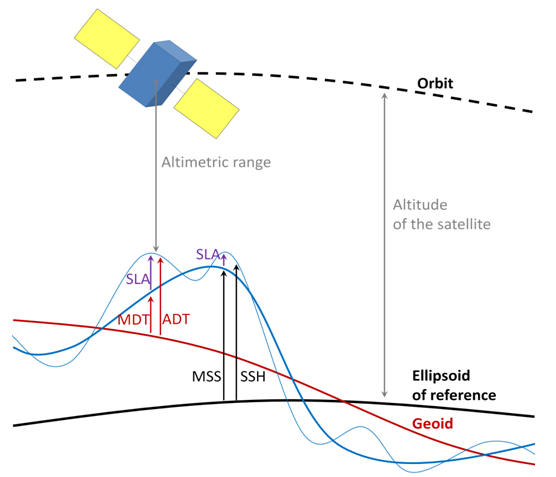
\includegraphics[width=\textwidth]{ABC_Altimetry.png}
   		\caption{BBB.
    	\label{fig:area_de_estudo_grade}}
	\end{figure}

\section{Variável obtida pelo modelo}
	
\bibliographystyle{coppe-plain}
\bibliography{biblio/biblio}
\addcontentsline{toc}{section}{Referências}

\end{document}
